%!TEX root = ../Pflichtenheft.tex

\chapter{Benutzeroberfläche}

In diesem Projekt wird grundsätzlich zwischen zwei verschiedene Benutzeroberflächen unterschieden:

\begin{itemize}
	\item \textbf{Das Sprachinterface:} Es besteht im Wesentlichen aus dem Mikrofon, einem Lautsprecher und einem Button, und dienen der Sprachein- und -ausgabe. Bei Betätigung des Buttons wird das Mikrofon aktiv und nimmt die gesprochene Sprache solange auf, bis die Stimme verstummt. Anschließend erfolgt nach der Verarbeitung der Spracheingabe die Ausgabe über die Lautsprecher. Sollte eine Nachfrage nötig sein, aktiviert sich das Mikrofon wieder automatisch und wartet auf die erneute Benutzereingabe. Login und Logout funktionieren ebenfalls über eine Spracheingabe mit dem jeweiligen Benutzernamen.
    \item \textbf{Das Webinterface:} Es besteht aus einer Website, auf welcher der Nutzer sich mit seinem Namen und seinem Passwort einloggen kann. Anschließend können die Feeds eingesehen, neue Feeds hinzugefügt und bestehende Feeds abgemeldet werden. Auch können durch Texteingabe Fragen an den \NewsGenie gestellt werden, sowie Antworten beziehungsweise Artikel vom Benutzer bewertet werden. Als Administrator bietet das Webinterface zusätzlich die Möglichkeit User zu löschen oder in deren Rolle zu schlüpfen, während normale Nutzer nur ihren eigenen Account löschen können.
\end{itemize}

\section{Sprachinterface}

\textbf{Hinweis:}
Aufgrund der fehlenden graphischen Benutzeroberfläche finden sich hier die Beispieldialoge, welche der \NewsGenie führen kann.

\textbf{Hinweis:}
Bei den folgenden Dialogen handelt es sich nicht um die endgültigen Sätze der Sprachausgabe. Änderungen sind vorbehalten.

\newpage

\begin{ui}{10}{Sprachinterface -- Dialog einer Anfrage}
Ein Beispiel für einen normalen Anfragedialog, in welchem \NewsGenie alles versteht. 
\smallskip\\
\begin{tabular}{|lp{0.85\linewidth}|}\hline
  User: & What's new in technology? \\
  \NewsGenie: & The latest news are: Android 4.4.3 is rolling out to Nexus 5, iOS will be connectable with cars from various 
  companies, Kim Dotcom wins back cars and cash and First Heartbleed 'hacker' arrested. Please say "`More"' for more news.\\
  User: & Tell me more about Android. \\
  \NewsGenie: & Android 4.4.3 is rolling out to all Nexus 5 from today. \ldots \\
  User: & And what about Apple? \\
  \NewsGenie: & \ldots \\
  \hline
 \end{tabular} 
\end{ui}
 
\pagebreak[2]

\begin{ui}{10}{Sprachinterface -- Dialog einer Anfrage mit einem Keyword, welches mehrmals auftaucht}
Ein Beispiel für einen normalen Anfragedialog, in welchem \NewsGenie alles versteht. 
\smallskip\\
\begin{tabular}{|lp{0.85\linewidth}|}\hline
  User: & What happens in the android scene? \\
  \NewsGenie: & I've found the following news: Android 4.4.3 is rolling out to Nexus 5. CyanogenMod shows first smartphone from OnePlus. Please say "`More"' for more news.\\
  User: & Tell me more about Android 4.4.3. \\
  \NewsGenie: & Do you mean Android 4.4.3 is rolling out to Nexus 5? \\
  User: & Yes \\
  \NewsGenie: & Android 4.4.3 is rolling out to all Nexus 5 from today.\ldots \\
  \hline
 \end{tabular} 
\end{ui}
 
\pagebreak[2]

\begin{ui}{11}{Sprachinterface -- Dialog einer Anfrage mit Nachfrage}
Ein Beispiel für einen normalen Anfragedialog, in welchem \NewsGenie nicht alles versteht und nachfragt. 
\smallskip\\
\begin{tabular}{|lp{0.85\linewidth}|}\hline
  User: & What happens in the Ukraine? \\
  \NewsGenie: & Sorry, I don't understand you. Please tell me again what you want to hear.\\
  User: & What happens in the Ukraine? \\
  \NewsGenie: & That's what I found for you: Overwhelmed, underfunded: why Ukraine isn’t retaliating, Russia in new Ukraine attack threat, \ldots \\
  User: & \ldots \\
  \hline
 \end{tabular} 
\end{ui}

\pagebreak[4]

\begin{ui}{12}{Sprachinterface -- Dialog einer Anfrage mit einer bestimmten Seite}
Ein Beispiel für einen normalen Anfragedialog, in welchem \NewsGenie alles versteht. 
\smallskip\\
\begin{tabular}{|lp{0.85\linewidth}|}\hline
  User: & Tell me, what's new on BBC.com? \\
  \NewsGenie: & Hamas and Fatah declare end to rift, Turkey: Armenia killings 'inhumane', Obama pledges Japan islands support and Iran replaces prison service chief. Please say "`More"' for more news.\\
  User: & Tell me the story about the armenia. \\
  \NewsGenie: & Turkey's Prime Minister Recep Tayyip Erdogan offers condolences for the first time for the mass killings of Armenians under Ottoman rule during WWI.\ldots \\
  User: & \ldots \\
  \hline
 \end{tabular} 
\end{ui}

\pagebreak[2]

\begin{ui}{13}{Sprachinterface -- Dialog einer Faktanfrage}
Ein Beispiel für einen normalen Anfragedialog, in welchem \NewsGenie alles versteht. 
\smallskip\\
\begin{tabular}{|lp{0.85\linewidth}|}\hline
  User: & Tell me, how old is President Obama? \\
  \NewsGenie: & President Obama is 52 years old.\\ \hline
 \end{tabular} 
\end{ui}

\pagebreak[2]

\begin{ui}{14}{Sprachinterface -- Dialog einer Anfrage auf Deutsch}
Ein Beispiel für einen normalen Anfragedialog, in welchem \NewsGenie alles versteht. 
\smallskip\\
\begin{tabular}{|lp{0.85\linewidth}|}\hline
  User: & Hi \NewsGenie, was gibt es neues rund ums Auto? \\ 
  \NewsGenie: & Wer wird Miss Tuning 2014?, BMW: Zwei Nummern größer, Liebesgrüße vom BMW X6, Super-Mustang zum Geburtstag. Wenn du mehr Nachrichten hören möchtest, sage "`Mehr"'.\\ 
  User: & Erzähl mir etwas über die Miss Tuning. \\ 
  \NewsGenie: & Am 4. Mai 2014 schauen die Fans gespannt zum Bodensee, wenn auf der Tuning World der Bär steppt und die Massen bei der Wahl zur Miss Tuning johlen. 20 Girls sind im Rennen, doch es gibt nur eine Krone.\ldots \\
  User: & \ldots \\ \hline
 \end{tabular}
\end{ui}

%\newpage

\section{Webinterface}

\textbf{Hinweis:} Bei den folgenden Abbildungen handelt es sich nicht um die endgültigen Darstellungen der Benutzeroberflächen.
Änderungen sind vorbehalten.

\begin{ui}{20}{Webinterface -- Login}
Der Login bietet ein Textfeld für den Benutzernamen und ein Passwortfeld, womit sich der Nutzer im Webinterface des \NewsGenies anmeldet. Über "`Register"' kann sich der Nutzer zusätzlich über \ref{UI21} registrieren. Mit einem Klick auf "`Forgot Password?"' gelangt man zusätzlich zu \ref{UI22}.
(Abbildung~\ref{fig:wi-login})
\begin{figure}[ht]
\centering
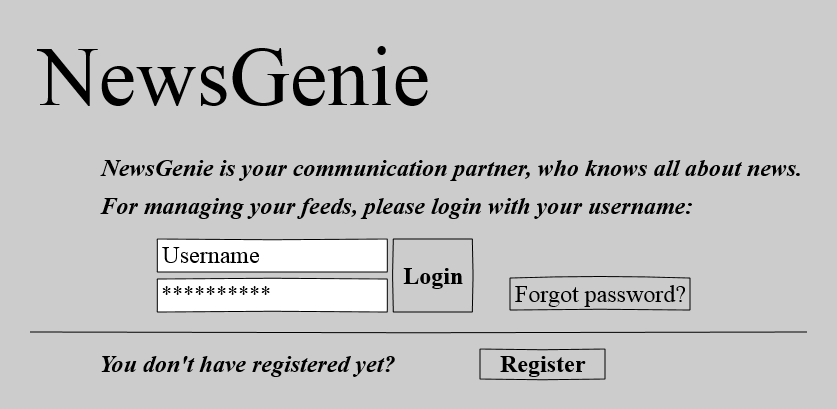
\includegraphics[width=0.8\linewidth]{figures/webinterfaceLogin.png}
\caption{\textit{Webinterface -- Login} \ref{UI20}}
\label{fig:wi-login}
\end{figure}
\end{ui}

\pagebreak[3]

\begin{ui}{21}{Webinterface -- Registrierung}
Bei der Registrierung muss der neue Nutzer einen Benutzernamen und ein Passwort wählen und seine E-mail-Adresse eintragen. Nach einem Klick auf "`Register"' ist der Nutzer registriert und kann sich anschließend mit seinem Benutzernamen und Passwort anmelden. (Abbildung~\ref{fig:wi-reg})
\begin{figure}[ht]
\centering
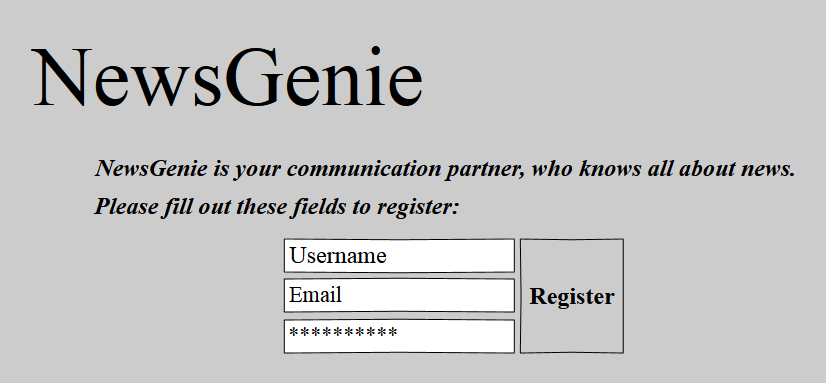
\includegraphics[width=0.8\linewidth]{figures/webinterfaceRegister.png}
\caption{\textit{Webinterface -- Registrierung} \ref{UI21}}
\label{fig:wi-reg}
\end{figure}
\end{ui}

\begin{ui}{22}{Webinterface -- Passwort vergessen}
Die "`Passwort vergessen"'-Funktion bietet dem Nutzer die Möglichkeit, sich ein neues Passwort mit Eingabe der E-mail-Adresse und des Benutzernamens zuschicken zu lassen.
(Abbildung~\ref{fig:wi-recpw})
\begin{figure}[ht]
\centering
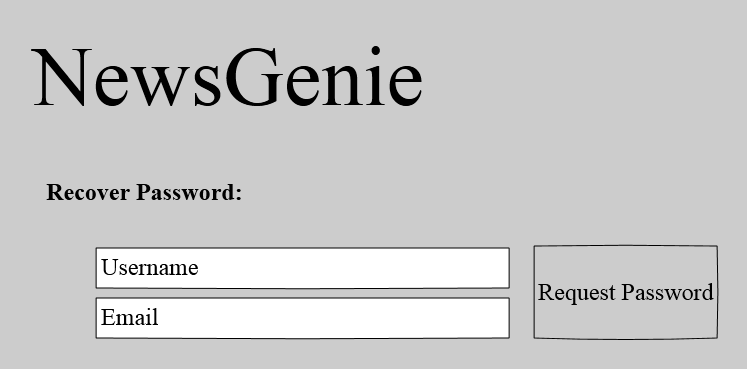
\includegraphics[width=0.8\linewidth]{figures/webinterfacePasswordRecover.png}
\caption{\textit{Webinterface -- Passwort vergessen} \ref{UI22}}
\label{fig:wi-recpw}
\end{figure}
\end{ui}

\pagebreak[4]

\begin{ui}{23}{Webinterface -- Passwort ändern und Account löschen} 
Die "`Passwort ändern"'-Funktion bietet den Nutzer die Möglichkeit, sich ein neues Passwort zu wählen. Dazu gibt er sein aktuelles und zweimal das neue Passwort ein und drückt auf "`Change Password"'. Zusätzlich kann der eigene Account hier gelöscht werden. (Abbildung~\ref{fig:wi-cpw})
\begin{figure}[ht]
\centering
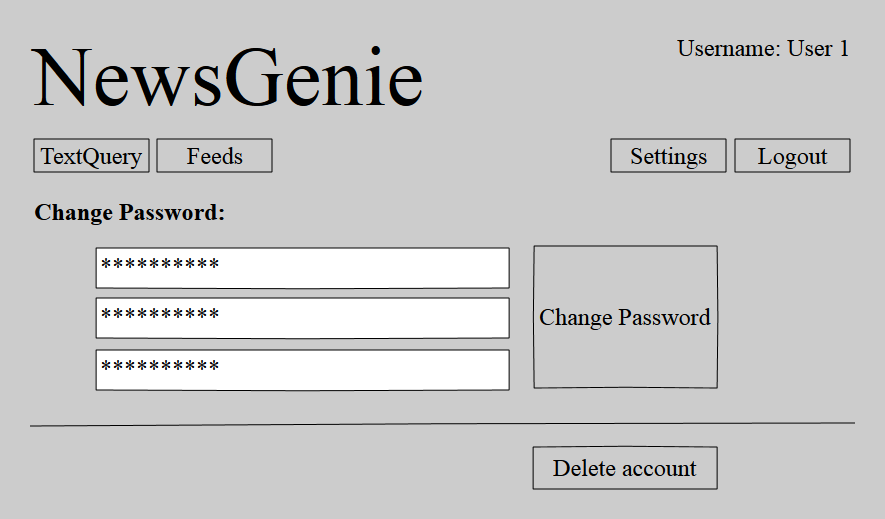
\includegraphics[width=0.8\linewidth]{figures/webinterfacePasswordChange.png}
\caption{\textit{Webinterface -- Passwort ändern und Account löschen} \ref{UI23}}
\label{fig:wi-cpw}
\end{figure}
\end{ui}

%\pagebreak[3]

\begin{ui}{30}{Webinterface -- Feedmanager}
Diese Ansicht zeigt eine Liste der vom Nutzer abonnierten Feeds und zwei Buttons sowie ein Texteingabefeld. Der Anwender kann für jeden Feed eine Markierung setzen, um anschließend die markierten Feeds abzubestellen. Über den Button "`Add"' können weiterhin RSS-Feeds neu abonniert werden.
(Abbildung~\ref{fig:wi-feedman})
\begin{figure}[ht]
\centering
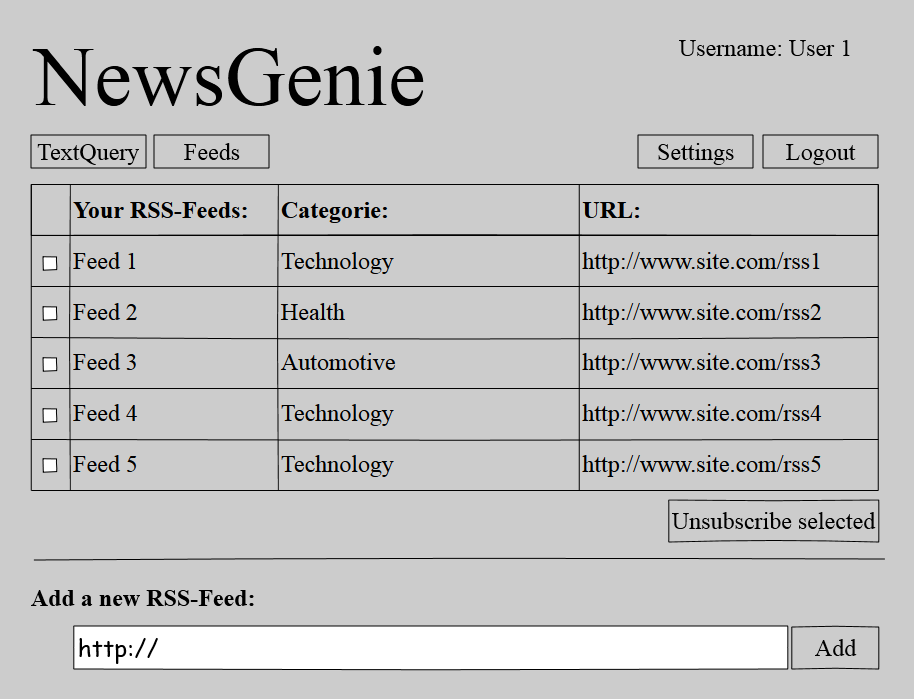
\includegraphics[width=0.8\linewidth]{figures/webinterfaceFeedManager.png}
\caption{\textit{Webinterface -- Feedmanager} \ref{UI30}}
\label{fig:wi-feedman}
\end{figure}
\end{ui}

%\pagebreak[3]

\begin{ui}{31}{Webinterface -- Textanfrage und Artikelbewertung}
Hier kann der Nutzer Textanfragen an das \NewsGenie stellen und Artikel für die Personalisierung seiner Nachrichten bewerten. Dabei steht ihm eine Skala von eins bis fünf zur Verfügung.
(Abbildung~\ref{fig:wi-textquery})
\begin{figure}[ht]
\centering
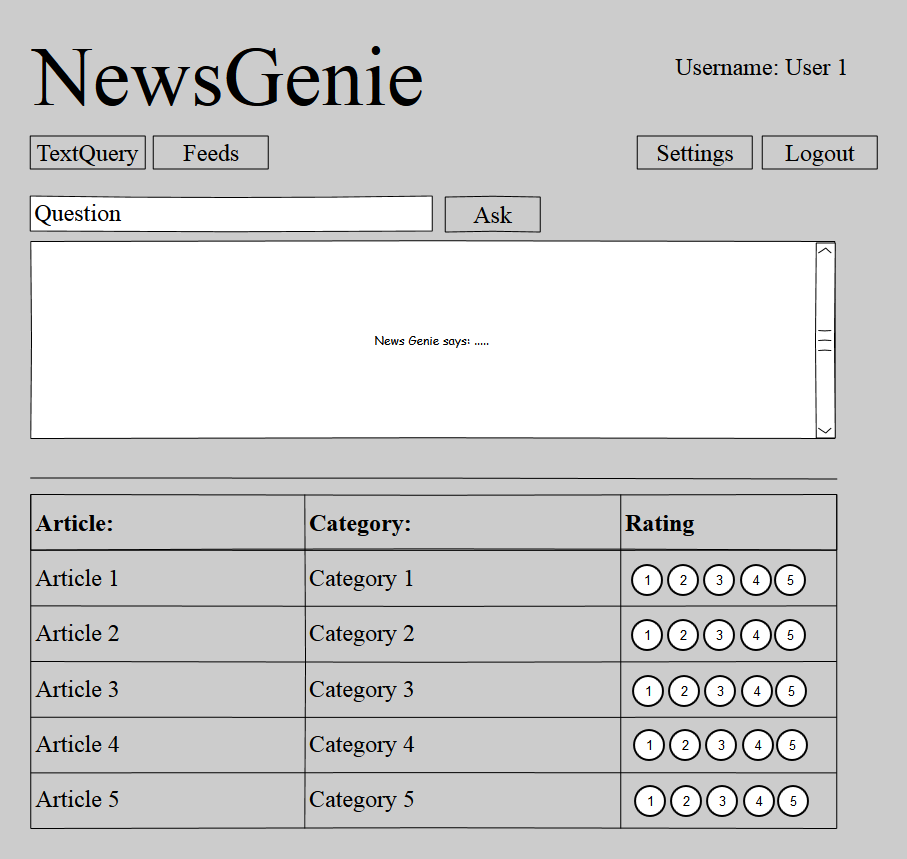
\includegraphics[width=0.8\linewidth]{figures/webinterfaceTextQueryArticleRating.png}
\caption{\textit{Webinterface -- Textanfrage und Artikelbewertung} \ref{UI31}}
\label{fig:wi-textquery}
\end{figure}
\end{ui}

%\pagebreak[3]

\begin{ui}{40}{Administratorenwebinterface -- Benutzer löschen}
\NewsGenie soll zudem Administratoren die Möglichkeit geben, andere User zu löschen. Dazu kann der Administrator jeden zu löschenden Benutzer markieren und anschließend per Klick auf den Button löschen. Weiterhin bietet das Admistratoren-Webinterface einen Button, mit welchem der Administrator in die Rolle des jeweiligen Benutzers wechseln kann.
(Abbildung~\ref{fig:wi-admin-deluser})
\begin{figure}[ht]
\centering
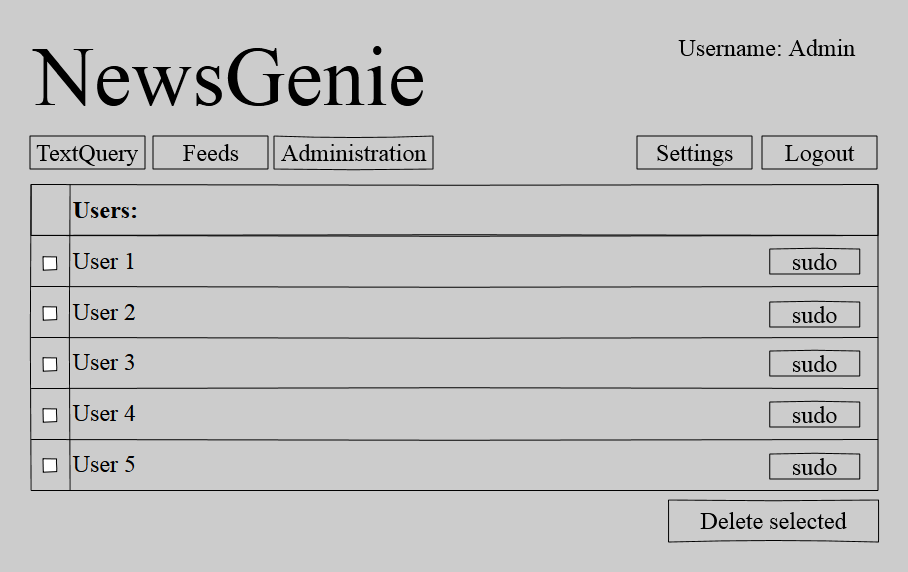
\includegraphics[width=0.8\linewidth]{figures/webinterfaceUserDelete.png}
\caption{\textit{Administratorenwebinterface -- Benutzer löschen} \ref{UI40}}
\label{fig:wi-admin-deluser}
\end{figure}
\end{ui}

